\chapter{Network Address Translation (NAT) and Firewall}
\section{}{Network Address Translation (NAT)}
\begin{itemize}
\item There are several situations where we need address translation such as, a network which do not have sufficient public IP addresses want to connect with the Internet, two networks which have same IP addresses want to merge or due to security reason a network want to hide its internal IP structure from the external world. NAT (Network Address Translation) is the process which translates IP address. NAT can be performed at firewall, server and router.
\item Network Address Translation allows a single device, such as a router, to act as an agent between the Internet (or "public network") and a local (or "private") network. This means that only a single, unique IP address is required to represent an entire group of computers.
\item In this session we are configuring Natting and also firewall
\end{itemize}

\begin{figure}[H]
\centering
  \includegraphics[width=0.9\textwidth]{Images/NAT & firewall experiment configuration.png}
  \caption{Nat and firewall experiment}
  \label{fig }
\end{figure}

\subsection{Network Address Translation (NAT)}
We consider our network D to be a private network and thus achieve that
balancer serves as an entry-point to gik.de. Therefore, we change the configuration in the following way.
We configure natting commands on router-2.
\begin{itemize}
\item To begin the natting we add a outbound interface command with Ethernet 0 
"set Nat source rule 10 outbound-interface eth0"
\item for a source NAT with the gateway 40.40.0.2/24 in network D, we use the following command "set Nat source rule 10  source address 40.40.0.0/24"
\item After adding source NAT with the gateway 40.40.0.2/24 in network D, we have to masquerade domain D to reach domains B, A and F so we use "set Nat source rule 10 translation address masquerade"
\end{itemize}
\begin{figure}[H]
\centering
  \includegraphics[width=0.8\textwidth]{Images/Natting commands .png}
  \caption{Natting commands on R2}
  \label{fig }
\end{figure}

\subsection{On r1 and r3 remove the route to reach collision domain (CD) D}
In this session we remove routing configuration from router-1 and router-3 so that we cannot reach collision domain D
\begin{figure}[H]
\centering
  \includegraphics[width=0.8\textwidth]{Images/Removing route to Collision domain D.png}
  \caption{Removing route}
  \label{fig }
\end{figure}

\subsection{From PC2 ensure that, e.g., web Sheldon is not pingable, but curl gik.de still delivers a result.}
\begin{itemize}
\item In this session our aim is to ensure that, web Sheldon is not pingable, but curl gik.de still delivers a result

\item If we try to ping Web Sheldon from Pc2 it is not reachable after removing the routes in R1 but curl gik.de still delivers a results .
\end{itemize}

\begin{figure}[H]
\centering
  \includegraphics[width=0.8\textwidth]{Images/web_sheldon is not pingable .png}
  \caption{web Sheldon is not pingable}
  \label{fig }
\end{figure}

\begin{figure}[H]
\centering
  \includegraphics[width=0.8\textwidth]{Images/web_sheldon is not pingable but curl gik.de still delivers a result.png}
  \caption{web Sheldon is not pingable but curl gik.de still delivers a result}
  \label{fig }
\end{figure}

\subsection{On CD B and CD D capture the call curl gik.de with wire shark and explain
the behaviour.}
\begin{itemize}
\item In this session we try to capture the packets on wire-shark by using curl gik.de see weather the natting we configured is working properly.
\item we have added natting on the collion D , hence we can observe the the router acts as a agent between the three web server's and other collision domain so This means that only a single, unique IP address is required to represent an entire group of computers.
\item Hence, all the three web servers, web-Sheldon, web-Howard and web-Leonard ip's will be mapped to the IP 40.40.0.2
\end{itemize}

\section{Firewall}
In this session we configure firewall On network E, we want to restrict the access to our servers and drop all packets except the ones, which establish tcp connections on port 80. Therefore, 
we need to enable a firewall with iptables on r3
Before we move further we run iptables on the router 3 and look for the output 
We use below command to check the firewall rules.
\begin{itemize}
\item iptables -L
\end{itemize}
\begin{figure}[H]
\centering
  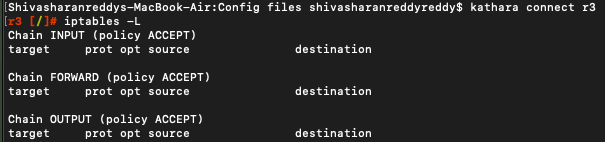
\includegraphics[width=0.8\textwidth]{Images/R3 before aplying any firewall rules .png}
  \caption{R3 before applying firewall rules}
  \label{fig }
\end{figure}
\subsection{we need to enable a firewall with iptables on r3.}
\subsubsection{(A) Create a default filter policy to drop all packets}
To drop all the packets entering network we use set of firewall iptables commands listed below on r3.
\begin{itemize}
\item iptables -F
\item iptables -X
\item iptables -P INPUT DROP
\item iptables -P OUTPUT DROP
\item iptables -P FORWARD DROP
\end{itemize}

\begin{figure}[H]
\centering
  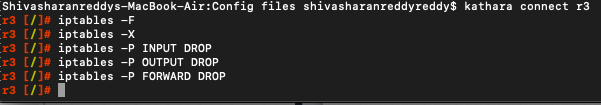
\includegraphics[width=0.8\textwidth]{Images/Firewall rules-01.png}
  \caption{  default filter policy to drop all packets}
  \label{fig }
\end{figure}

So, after we configure these commands on R3 we have to use iptables -L on R3 and check if all the packets are been dropped.
We can see in the below figure that all the packets are dropping.
\begin{figure}[H]
\centering
  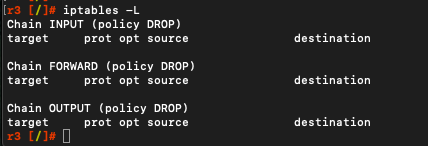
\includegraphics[width=0.8\textwidth]{Images/Packets dropped .png}
  \caption{Packets are dropped}
  \label{fig }
\end{figure}

\subsubsection{(B) Allow unlimited traffic on the loop-back interface lo again.}
To allow unlimited traffic on the loop-back interface lo we use following set of commands.
We have two commands for loop back interface, one for input and another for output.
\begin{itemize}
\item iptables -A INPUT -i lo -j ACCEPT
\item iptables -A OUTPUT -o lo -j ACCEPT
\end{itemize}

\begin{figure}[H]
\centering
  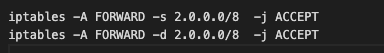
\includegraphics[width=0.8\textwidth]{Images/Loopback interface commands .png}
  \caption{Loop back interface firewall commands}
  \label{fig }
\end{figure}
After we configure these commands on r3 we use iptables -L to check if the firewall is allowing unlimited traffic on the loop back interface lo.
\begin{figure}[H]
\centering
  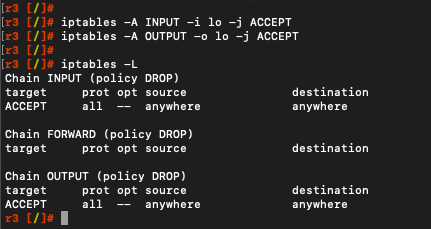
\includegraphics[width=0.8\textwidth]{Images/allowing Afterunlimited traffic on the loopback interface lo.png}
  \caption{Allowing traffic on lo interface}
  \label{fig }
\end{figure}

\subsubsection{(C) Forward packets of the DNS network 2.0.0.0/8 without any restrictions.}
To forward packets of the DNS network 2.0.0.0/8 without any restrictions we configure two commands on r3, one for source address and another for Destination.
\begin{itemize}
\item iptables -A FORWARD -s 2.0.0.0/8  -j ACCEPT
\item iptables -A FORWARD -d 2.0.0.0/8  -j ACCEPT 
\end{itemize}

\begin{figure}[H]
\centering
  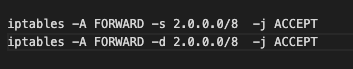
\includegraphics[width=0.8\textwidth]{Images/Firewall commands -03.png}
  \caption{Firewall commands -03}
  \label{fig }
\end{figure}
After we configure these commands on r3 we use iptables -L to check if the firewall is 
Forwarding packets of the DNS network 2.0.0.0/8 without any restrictions.
\begin{figure}[H]
\centering
  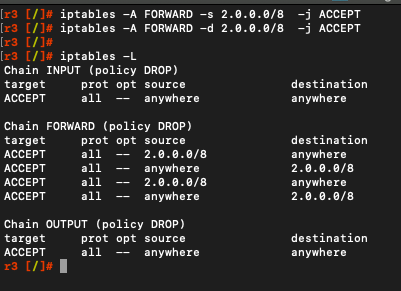
\includegraphics[width=0.8\textwidth]{Images/Forward packets of the DNS network 2.0.0.0:8 without any restrictions..png}
  \caption{Forward packets of the DNS network}
  \label{fig }
\end{figure}

\subsubsection{(D) Allow all web servers in CD E to accept connections on tcp port 80.}
To Allow all web servers in CD E to accept connections on tcp port 80, we configure two commands on r3, one for source address and another for Destination.
\begin{itemize}
\item iptables -A FORWARD -d 50.50.0.0/25 -p tcp --dport 80 -j ACCEPT 
\item iptables -A FORWARD -s 50.50.0.0/25 -p tcp --sport 80 -j ACCEPT 
\end{itemize}

\begin{figure}[H]
\centering
  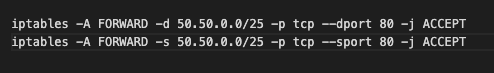
\includegraphics[width=0.8\textwidth]{Images/Firewall commands -04.png}
  \caption{Firewall commands-04}
  \label{fig }
\end{figure}
After we configure these commands on r3 we use iptables -L to check if the firewall is Allowing all web servers in CD E to accept connections on tcp port 80.
\begin{figure}[H]
\centering
  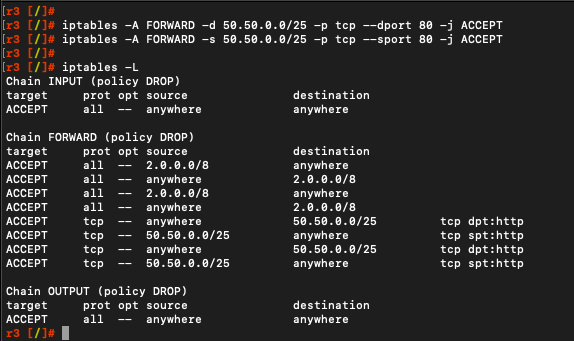
\includegraphics[width=0.8\textwidth]{Images/Allow all web servers in CD E to accept connections on tcp port 80.png}
  \caption{Allowing all web servers in CD E to accept connections on tcp port 80}
  \label{fig }
\end{figure}

\subsection{On PC2 ensure that ping gik.org fails, but curl gik.org displays the website content.}
After all the configuration on r3 we need to connect PC1 and check if it full-fills all requirements, ping gik.org should fail but curl gik.org displays the website content.
As we can see ping gik.org is failing on PC1 as we configured in firewall rules but curl gik.org should should display website content as shown below.
\begin{figure}[H]
\centering
  \includegraphics[width=0.8\textwidth]{Images/Curl gik org is displaying website content.png}
  \caption{ping gik.org is failing but curl gik.de is displaying website content on pc2}
  \label{fig }
\end{figure}

